\begin{frame}[allowframebreaks]
	\par The liquid state machine (LSM) has emerged as a computational model that is more suitable than Turing machines for describing neural networks. It is used to process continuous streams of data, typically in the form of spike trains, and it maps streams of inputs into streams of outputs. These outputs may depend on the previous states created by the streaming data \cite{doi:10.1142/9781848162778_0008}.
	
	\par LSM is model for adaptive computing systems. Considering that the training stage is the most expensive and sensible one, these kind of networks are trained only at the readouts. These readouts, usually, consists of only a single neuron which is called \textit{"projection neuron"} that extracts information from a micro-circuit somewhere in the LSM. These structures can be used as inputs to another area of the neural network and can be modeled as a perceptron, linear gate, sigmoidal gate, spike neuron and others \cite{doi:10.1142/9781848162778_0008}. The networks structure consists of several neurons randomly and recurrently connected forming the \textit{"liquid part"} which is interpreted by the readouts. The word \textit{"liquid"} can sometimes be take literally like in this work \cite{10.1007/978-3-540-39432-7_63} where a bucket of water has been taken the role of the liquid part of the network as can be seen in Figure \ref{fig:leterallyaliquidnetwork}.
	
	\begin{figure}
		\centering
		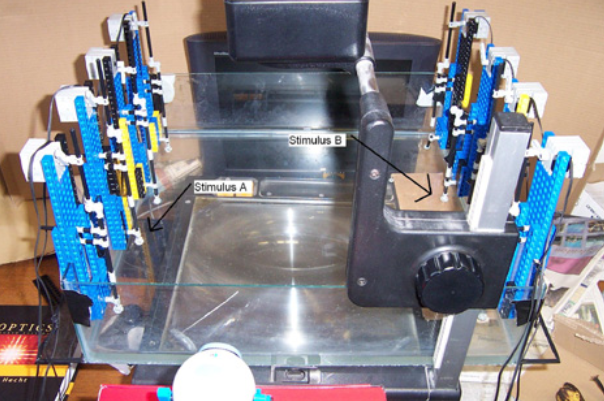
\includegraphics[width=0.7\linewidth]{images/leterallyALiquidNetwork}
		\caption[A liquid network]{A liquid network. Source: \cite{10.1007/978-3-540-39432-7_63}}
		\label{fig:leterallyaliquidnetwork}
	\end{figure}
	
	\par LSM can be adapted to multiple computation as the projection neurons can extract as many different characteristics one desires as can be seen in Figure \ref{fig:projectionneurons}.
	
	\begin{figure}
		\centering
		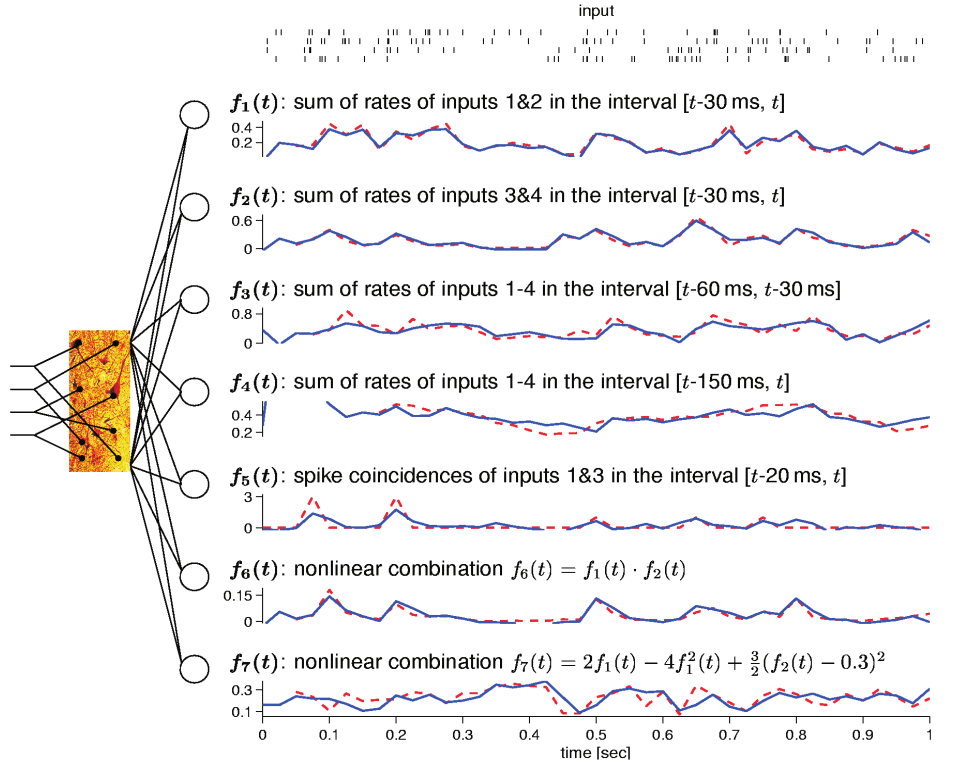
\includegraphics[width=0.7\linewidth]{images/projectionNeurons}
		\caption{}
		\label{fig:projectionneurons}
	\end{figure}

\end{frame}

\section{More liquid}

\begin{frame}[allowframebreaks]
	
	\par Also, according to \cite{hasani2020liquid} the inspiration comes from the nervous system of the nematode \textit{C. elegans} which, despite having just 302 neuron, have pretty complex behavior. In this model the networks parameter changes over time according to a set of nested differential equations \textbf{while it is already in use} i.e. \textbf{this model does not need a training phase in order to adapt}.
	
	\par Conversely, LNNs introduce dynamic connectivity patterns, allowing information to flow and interact in a fluid manner.
	
	\par Liquid Neural Networks, also known as Liquid State Machines (LSMs), were first introduced by Wolfgang Maass\cite{6789852}. The primary departure from traditional ANNs lies in their dynamic and recurrent architecture. While conventional ANNs consist of fixed layers of interconnected neurons, LNNs employ a vast collection of interconnected neurons that are constantly in a state of change. This dynamic behavior allows LNNs to process temporal data, sequential information, and streaming inputs with remarkable flexibility and efficiency.
	
	\begin{itemize}
		\item Adaptability: Their dynamic nature enables them to respond dynamically to varying data distributions, making them well-suited for tasks involving non-stationary data.
		\item Robustness: LNNs have shown improved robustness against noise and input variations. The fluid-like behavior allows them to self-adjust and filter out irrelevant information, leading to enhanced generalization capabilities.
		\item Exploration of Solution Space: LNNs encourage solution space exploration by providing flexibility in the network’s structure. The dynamic connectivity patterns enable the network to explore diverse pathways, potentially discovering novel solutions to complex problems.
		\item Reduced Overfitting: Due to their continuous learning capabilities, LNNs are less prone to overfitting, which often occurs in static networks, resulting in more accurate and generalizable models.
	\end{itemize}
	
	\par Being $f$ the neural network, $I(t)$ its inputs, $t$ current time, $\theta$ and $A$ the hiperparameters and $\tau$ is time constant than the equation \ref{eq:liquidRNN} represents the Liquid Time-Constant recurrent neural networks (LTC) hidden state's derivative \cite{hasani2020liquid}.
	
	\begin{equation}
		\label{eq:liquidRNN}
		\dfrac{d x(t)}{dt} = - \left[\dfrac{1}{\tau} + f(x(t),I(t), t, \theta)\right] x(t) + f(x(t),I(t), t, \theta) A \qquad.
	\end{equation}
	
	\par To simplify a neuron in these kind of networks can be expressed like in the listing .
	
	\input{listings/LiquidTimeConstantNeuron.py}
	
	
\end{frame}